\chapter{INTRODUÇÃO}
\label{chap:intro}
Para obter a construção do melhor modelo de helicóptero a base de papel, produzido seguindo o modelo da figura \ref{fig:modeloA4}, impresso no papel A4, a equipe borgs, desenvolveu um protótipo e realizou alguns lançamentos do modelo citado para analisar sua eficiência, avaliar qual a melhor configuração para que o modelo permaneça mais tempo no ar e analisar quais características podem interferir no desempenho de sua função. Após finalizado os lançamentos, foi gerada uma tabela com os tempos de lançamento de cada experimento.  A partir daí, foi realizada uma análise estatística utilizando o software R, no qual foi gerada as tabelas de comportamento gerado pela variação da altura e dos tipos de configuração física do protótipo.

\begin{figure}[H]
    \centering
    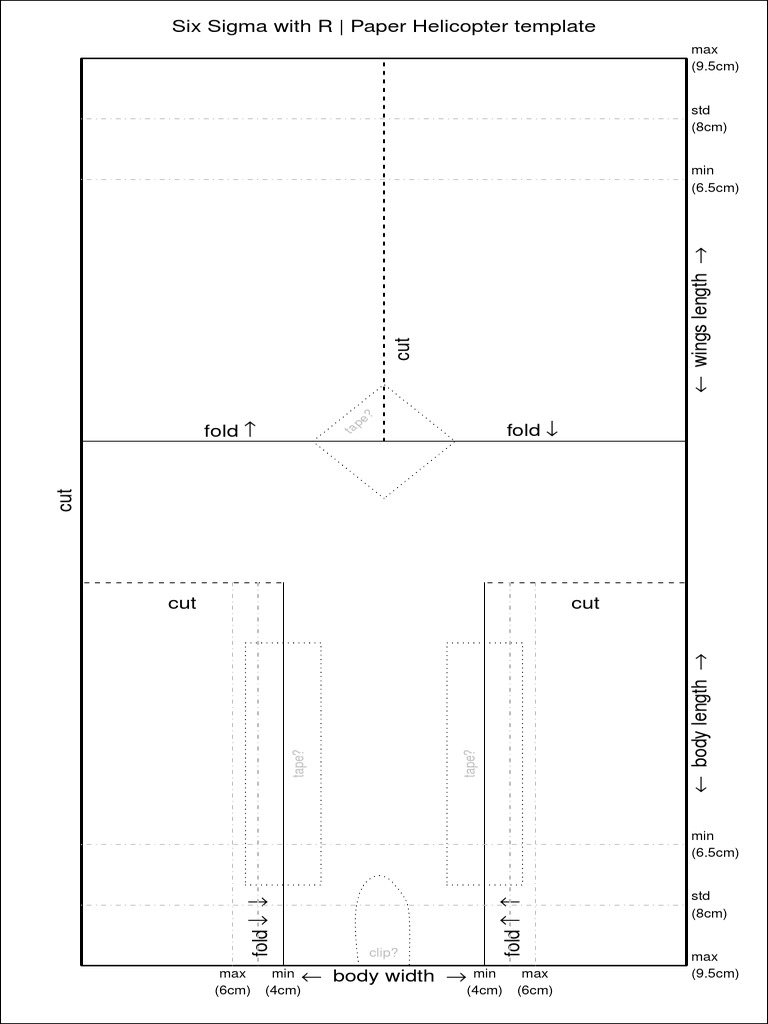
\includegraphics[scale=0.4]{images/helicoptero.jpeg}
    \caption{Cadeia de suprimentos.}
    \label{fig:modeloA4}
  \end{figure}

%------------------------------------------------------------------

\section{Objetivos}
\label{sec:obj}
Este trabalho tem como objetivo principal a criação, desenvolvimento e analise de um helicóptero impresso. O estudo do comportamento estatístico do modelo analisado, modelo matemático de tendência, repetitividade e reprodutividade foram feitos para aplicação e confirmação do experimento proposto.

%------------------------------------------------------------------
\section{Organização do relatório}
\label{sec:org}
Este documento está organizado da seguinte forma:
\begin{enumerate}
    \item Descrição do experimento, explicação da construção do modelo, análise e coleta de dados, padronização do teste e as variações que foram aplicadas; 
    \item Primeiro experimento, descrição das coleta de dados, tomada e aplicação em uma tabela;
    \item Modelagem matemática, aplicação dos dados coletados em um modelo matemático, explicação do que foi usado para análisar e o que foi gerado da analise feita;
    \item Segundo experimento, descrição das coleta de dados, tomada e aplicação em uma tabela;
    \item Verificação do experimento, confirmação dos dados;
    \item Conclusão, compreensão sobre o trabalho que foi apresentado.
    
\end{enumerate}